\cotefile{157-5}
\scanpage{197}
\mspage{113}
% archive sheet number: 196
% element: text | top, lines 1-3 | une famille
une famille d'\unsure{éléments|objets} de $I$, elle est majorée par un $\unsure{j|J}\in I$. Ceci résulte du

% element: text | upper and middle, lines 4-11 | Lemme 4.5.5.
\uline{Lemme} 4.5.5. \inserted{\unsure{Soient} $\pi,\pi_0$, avec $\pi\unsure{\geq|>}\pi_0$, des cardinaux infinis, et} Soit $J$ une catégorie grande devant $\pi_0$. Alors pour \unsure{tte} partie $\unsure{K|\mathscr K}$ de $\mathrm{Fl}\,J$, telle que $\operatorname{card}K\leq\pi$, il existe une sous-catégorie $J'$ de $J$ \uline{grande devant $\pi_0$}, telle que $\operatorname{card}J'\leq\pi^{\unsure{*}}$, et \deleted{\unsure{$K$}} $\mathrm{Fl}\,J'\supset K$.
% slanted
% element: margin note | left of lemma, descending along edge | N'est prouvé
\margin{\unsure{N'est prouvé} \uuline{que} si $\pi^{\pi_0}=\pi$ \unsure{(sinon|simplement} \unsure{prendre|pour} \unsure{$\pi_0$}\unsure{?)}. \uuline{\unsure{Oui|fini?}}. C'est OK si \deleted{\unsure{l'on}} on \unsure{remplace} $\operatorname{card}J'\leq\pi^{\pi_0}$.}
\margin{\unsure{?}}

% element: text | middle to foot, lines 12-27 | Ce lemme
\deleted{\unsure{Démonstration}} Ce lemme étant admis, on \unsure{saura} \unsure{représenter|représenté} un objet quelc. $F$ de $M$, comme une $\varinjlim_{i\in I}X_i$, avec $I$ ensemble ordonné \unsure{grd|grand} devant $\pi$, les $X_i$ dans $\mathrm{Filt}^{\pi}$. Je note : \unsure{prouvons} que si $\pi'>\pi$ et $F\in\mathrm{Filt}^{\unsure{\pi|\pi'}}$, alors on pourra prendre $I$ tel que $\operatorname{card}I\leq\pi'{}^\pi$. Mais \deleted{\unsure{si}} $F\in\mathrm{Filt}^{\pi}$ signifie que $J=C_{/F}$ satisfait $\operatorname{card}\mathrm{Fl}\,J\leq\pi'$. Alors l'ens des parties de cardinal $\leq\pi$ de $\mathrm{Fl}\,J$ \deleted{est majoré par} a un cardinal majoré par $\pi'{}^\pi$, a fortiori $\operatorname{card}I\leq\pi'{}^\pi$ ce qui \unsure{achève de prouver} que $(\mathrm{Filt}^{\unsure{\pi'|\pi}})_{\pi\geq\pi_0}$ est une filtration cardinale sur $M$

\scanpage{198}
\mspage{114}
% archive sheet number: 197
% element: text | upper third, lines 1-10 | Pour prouver le lemme
Pour prouver le lemme, on commence par saturer $\unsure{K|\mathscr K}$ par composition finie, on trouve une sous-catégorie $J'_0$ de $J$ telle que $\operatorname{card}\mathrm{Fl}\,J'_0\leq\pi$. \unsure{\ldots} Mais je m'aperçois que pour prouver le lemme, j'ai encore besoin de $\pi^{\pi_0}=\pi$ --- \deleted{\unsure{je}} \inserted{car} les diagrammes de $J'$ \deleted{\unsure{filtrants par}} \unsure{petits} \unsure{d'ordre} $\pi_0$ ont un cardinal majoré (au mieux) par $\pi^{\pi_0}$.

% element: text | middle, lines 11-15 | Prenons p. ex.
Prenons p. ex. \deleted{\unsure{$S$}} (ens. ordonné)
% element: display | middle, line 12 | J = P(S)
\[
J=\unsure{\mathscr{P}|\mathfrak{P}|\mathrm{P}}(S)
\]
avec $\operatorname{card}S=\pi>\pi_0$, donc $J$ est grand devant $\pi_0$. Considérons l'injection
% element: display | middle, line 16 | S to J
\[
S\unsure{\lhook\joinrel\longrightarrow|\longrightarrow}J=\mathscr{P}(S),\qquad s\longmapsto\{s\},
\]
% element: text | lower half, lines 17-25 | et prenons pour K
et prenons pour $K$ \inserted{$\in\mathrm{Fl}\,J$} l'ens des $\mathrm{id}_{\{s\}}$. Donc on \unsure{demande|cherche} une partie $J'$ de $J$, contenant $S$, et grande devant $\pi_0$ \inserted{pour l'ordre induit par $J$}. On voit tout de suite que le plus petit $J'$ faisant l'affaire est l'ens. $\mathscr{P}_{\pi_0}(S)$ des parties de $S$ de cardinal $\leq\pi_0$. Mais \deleted{\unsure{card}} \unsure{on a}
% element: deletion | foot, first line of calculation | card J' times card Aut
\deleted{$\operatorname{card}J'\times\operatorname{card}(\unsure{\mathrm{Aut}}\text{ d'un ens }E_0\text{ de cardinal }\pi_0)=$}
% element: display | foot, last line | card J' pi0 factorial
\[
\operatorname{card}J'\cdot\deleted{\unsure{\times}}\pi_0!=\pi^{\pi_0}
\]

\scanpage{199}
\mspage{115}
% archive sheet number: 198
% element: text | top, line 1 | où
où
% element: display | top, lines 2-3 | pi0 factorial
\[
\begin{aligned}
\pi_0!&=\operatorname{card}\mathrm{Aut}\unsure{E_0)|(E_0)},\qquad E_0\text{ ens de cardinal }\pi_0\\
&=\pi_0^{\pi_0}=2^{\pi_0}
\end{aligned}
\]
% element: text | upper third, line 4 | donc
donc
% element: display | upper third, line 4 | card J' times two
\[
\operatorname{card}J'\cdot2^{\pi_0}=\pi^{\pi_0},
\]
% element: text | upper third, line 5 | or
or
% element: deletion | upper third, lines 6-7 | ce qui implique
\deleted{ce qui \unsure{implique}, \deleted{\unsure{pour}} si $\pi^{\deleted{\unsure{\pi_0}}}>2^{\pi_0}$, d'où $\pi^{\pi_0}>2^{\pi_0}$, que l'on a $\operatorname{card}J'>2^{\pi_0}$, \unsure{donc}}
% element: text | middle, lines 8-13 | D'autre part
D'autre part il est immédiat que $\operatorname{card}J'\geq\operatorname{card}\unsure{\mathscr P|\mathfrak P|\mathrm P}(E_0)=2^{\pi_0}$ (si $E_0$ est une partie de $S$ de cardinal $\leq\pi_0$), d'où le \deleted{\unsure{deuxième}} premier mb de ces égalités $\unsure{=|\text{à}}\operatorname{card}J'$, donc on trouve
% element: display | middle, line 14 | card J'
\[
\operatorname{card}J'=\pi^{\pi_0},
\]
% element: margin note | left beneath calculation | sorry!
\margin{\unsure{sorry!}}
% element: drawing | centre beneath calculation | short oblique separating stroke
\figure{\begin{tikzpicture}\draw (0,0.2)--(0.35,0);\end{tikzpicture}}

% element: text | lower half, lines 15-21 | Finalement
Finalement, je me suis convaincu que la prop. \unsure{4.5.3|4.5.2}, et les Corollaires et lemmes précédents par lesquels j'ai essayé de l'établir, \unsure{n'est vrai} que pour \deleted{\unsure{n'admet que pour les cardinaux}} \inserted{les cardinaux $\pi>\pi_0$ tels que} \deleted{$\pi\unsure{\geq|>}\pi_0$}
% element: display | lower half, line 21 | pi power pi0 equals pi
\[
\pi^{\pi_0}=\pi,
\]
% element: text | foot, lines 22-23 | ce qui moyennant
ce qui, moyennant l'hypothèse des continus \unsure{généralisée|généralisés}, équivaut à :
% element: display | foot, line 24 | pi power pi0 relation to two power pi
\[
\pi^{\pi_0}\unsure{<|\neq}2^\pi\ (=\pi^\pi)
\]
% element: text | foot, last line | ou mieux
(ou mieux : $\pi^{\pi_0}\neq2^\pi\ (=\pi^\pi)$). Je vais donner

\scanpage{200}
\mspage{116}
% archive sheet number: 199
% element: text | top, line 1 | ici un énoncé rectifié
\unsure{ici} un énoncé rectifié.

% element: text | upper third, lines 2-9 | Proposition 4.5.5
\uline{Proposition} \unsure{4.5.5|4.5.6} \textcircled{$1^\circ$} Dans les hypothèses générales de 4.5.2, \deleted{\unsure{des card}} $C,\pi_0,\pi_1,\pi$, les conditions $\unsure{a'|a''},b,c'$ de \deleted{loc. cit.} cette proposition sont équivalentes \inserted{[moyennant $\pi\geq\pi_1$]}, et impliquent la condition ($F$ est $\pi$-accessible). Quand $\pi^{\pi_0}=\pi$ (notamment quand $\pi=2^{\unsure{c|\sigma}}$, avec $c\geq\pi_0$), alors toutes les conditions \unsure{a) à i')} de 4.5.2 sont équivalentes.

% slanted
% element: margin note | diagonal left margin beside heading and first paragraph | NB Pour cette équivalence
\margin{\uline{NB} Pour cette équivalence, l'hyp que $C$ soit stable par $\varinjlim$ de card. $\leq\pi_0$ est inutile, et aussi \deleted{\unsure{(quand} $\pi^{\pi_0}=\pi$)} \deleted{\unsure{d'après le lemme}} \unsure{l'implication} \unsure{c)}, et l'équival. si $\pi=\pi^{\pi_0}\geq\pi_1$, \unsure{cf.} \unsure{4.7.1} (p.\unsure{161|151}). \unsure{(a'|c')} \unsure{et} \unsure{c)}\unsure{?}}

% element: text | middle, lines 9-12 | Plus généralement et plus précisément
\textcircled{$2^\circ$} Plus généralement et plus précisément, \deleted{\unsure{avec}} pour $\pi\geq\pi_0$ donné, \deleted{\unsure{les relations}} considérons les conditions sur $\pi$
\begin{enumerate}[label=\arabic*)]
% element: display | middle, item 1 | pi power pi0 equals pi
\item $\pi^{\pi_0}=\pi$
% element: text | middle, item 2 | Filt pi M
\item $\mathrm{Filt}^{\pi}(M)$ (défini dans 4.5.3) est stable par $\varinjlim$ de cardinal $\leq\pi$
% element: text | lower middle, item 3 | for all F in M
\item $\forall F$ dans $M$, on a $F\simeq\varinjlim_I X_i$, avec $I$ ens. ordonné grand devant $\pi$, les $X_i$ dans $\mathrm{Filt}^{\pi}(M)$. De plus, si $\pi'>\pi$ et $F\in\mathrm{Filt}^{\pi'}(M)$, on peut prendre $I$ de cardinal $\leq\unsure{\pi^{\pi^*}|\pi^{\pi'}|\pi'{}^{\pi}|\pi'{}^{\pi_0}}$.
% element: text | lower third, item 4 | Comme 3
\item Comme 3), sans la majoration de cardinaux, et \deleted{\unsure{avec}} en supposant seulement $I$ catégorie \unsure{grd|grde|grand} devant $\pi$ (pas néc. cat. ordonnée)
% element: text | foot, item 5 | La condition c
\item La condition c) de 4.5.2 implique les autres conditions (elles sont équivalentes, par $1^\circ$), en d'autres termes
% element: display | foot | M pi subset Filt pi
\[
M_\pi\subset\mathrm{Filt}^{\pi}\qquad(\text{donc }M_\pi=\mathrm{Filt}^{\pi}\text{ puisque}
\]
\unsure{on sait} que $\mathrm{Filt}^{\pi}\subset M_\pi$)
\end{enumerate}

\scanpage{201}
\mspage{117}
% archive sheet number: 200
% element: text | top, lines 1-3 | où M pi désigne
où $M_\pi$ désigne la sous-catégorie str. pleine de $M$ formée des objets $\pi$-accessibles.
Ceci posé, on a les implications
% element: diagram | upper third, line 4 | 1 implies 2 implies 3 implies 4 implies 5
\diagram{\begin{tikzcd}[ampersand replacement=\&]
1)\arrow[r,Rightarrow]\&2)\arrow[r,Rightarrow]\&3)\arrow[r,Rightarrow]\&4)\arrow[r,Rightarrow]\&5),
\end{tikzcd}}
% element: text | upper third, lines 5-8 | et dans le cas particulier
et dans le cas particulier où $M=(\mathrm{Ens})$, $C=$ sous-catégorie pleine formée des ensembles de cardinal $\leq\pi_0$, on a aussi $5)\Rightarrow1)$ i.e. toutes ces conditions sont équivalentes.

% element: text | middle, line 9 | Dém 1 implies 2
\uline{Dém.}\quad $1)\Rightarrow2)$, cf dém. de 4.5.4.

% element: text | middle, lines 10-18 | 2 implies 3 La catégorie
$2)\Rightarrow3)$ La catégorie $J=\mathrm{Filt}^{\pi}_{/F}$ est stable par $\varinjlim$ de cardinal $\leq\pi$, $\mathrm{Filt}^{\pi}$ l'étant, donc $J$ est \unsure{grande|grand} devant $\pi$, d'ailleurs $F=\varinjlim_{j\in J}X_j$, \unsure{dont|où} $j\longmapsto X_j$ est le foncteur source $\mathrm{Filt}^{\pi}_{/F}\longrightarrow\mathrm{Filt}^{\pi}$. \unsure{D'où|D'ou} la repr. voulue de $F$, quitte à remplacer $J$ par un ens ordonné cofinal $\unsure{I|\bar I}$, p.ex. en prenant pour $I$ l'ens des sous-catégories \deleted{\unsure{filtrantes de}} \deleted{\unsure{filtrantes}} $J$ de $I$ \deleted{de cardinal} \deleted{grandes devant $\pi$} \deleted{$\leq\pi$} telles que $\operatorname{card}\mathrm{Fl}\,J\leq\pi$. La majoration $\operatorname{card}I\leq\pi'{}^\pi$, pour $F\in\mathrm{Ob}\,\mathrm{Filt}^{\pi'}$, se fait par AQT.

% element: text | lower third, line 19 | L'implication 3 to 4
L'implication $3)\longrightarrow4)$ est tautologique

% element: text | foot, lines 20-23 | 4 implies 5
$4)\Rightarrow5)$, car si $F\in\mathrm{Ob}\,M_\pi$, on \unsure{trouve|tire} par 4) que $F$ est facteur direct d'un objet de $\mathrm{Filt}^{\pi}$, et $\mathrm{Filt}^{\pi}$ étant stable par $\varinjlim$
% slanted
% element: margin note | bottom left, beside 4 implies 5 | Comparer le lemme
\margin{Comparer le lemme 4.5.14 \unsure{page|pg} 133}

\scanpage{202}
\mspage{118}
% archive sheet number: 201
% element: text | top, lines 1-4 | grandes devant pi0
grandes devant $\pi_0$, cela implique que $\mathrm{Filt}^{\pi}$ est stable par facteurs directs, d'où $F\in\mathrm{Ob}\,\mathrm{Filt}^{\pi}$.

Enfin, si $M=\mathrm{Ens}$, $C=\unsure{\mathrm{Ens}(\leq\pi_0)|\mathrm{Ens}(\pi_0)}$. On note que
% element: display | upper third, line 5 | Filt pi equals set
\[
\mathrm{Filt}^{\pi}=\{X\in\mathrm{Ob}\,\mathrm{Ens}\mid\operatorname{card}(X)^{\pi_0}\leq\pi\}
\]
% element: text | upper middle, line 6 | D'autre part
D'autre part, on trouve facilement
% element: display | upper middle, lines 7-9 | Ens pi definition
\[
\begin{aligned}
(\mathrm{Ens})_\pi&\overset{\mathrm{def}}=\text{sous-catégorie pleine de }(\mathrm{Ens})\text{ formée}\\
&\qquad\text{des objets }\pi\text{-accessibles}\\
&=\{X\in\mathrm{Ob}\,\mathrm{Ens}\mid\operatorname{card}X\leq\pi\}
\end{aligned}
\]
% element: text | middle, lines 10-11 | Donc on a
Donc on a $(\mathrm{Ens})_\pi\subset\mathrm{Filt}^{\pi}$ ssi $\pi^{\pi_0}\leq\pi$, i.e. $\pi^{\pi_0}=\pi$, qed.
% element: margin note | right of conclusion, above corollary | Cf démonstration
\margin{Cf. \deleted{\unsure{faite}} \inserted{démonstration} de \unsure{la|(la} partie $1^\circ$) de 4.5.6, plus bas. (\unsure{fin de page} et p. suivante)}

% element: text | middle, line 12 | Corollaire 4.5.7
\uline{Corollaire 4.5.7}. Pour tt cardinal $\pi\geq\pi_1$, on a
% element: display | middle, line 13 | Filt pi subset M pi subset Filt
\[
\mathrm{Filt}^{\pi}\subset M_\pi\subset\mathrm{Filt}^{\pi^{\pi_0}}
\tag*{(4.5.7.1)}
\]
% element: text | lower half, lines 14-23 | L'inclusion
L'inclusion $\mathrm{Filt}^{\pi}\subset M_\pi$ est l'implication $a\Rightarrow c$ de la partie $1^\circ$ de 4.5.6. Pour prouver $M_\pi\subset\mathrm{Filt}^{\pi^{\pi_0}}$, \unsure{on|en} \deleted{étant noté que} \inserted{pose $\pi'=\pi^{\pi_0}$ et} \deleted{$\pi'$} on note que $\pi'{}^{\pi_0}=\pi^{\pi_0\cdot\pi_0}=\pi^{\pi_0}=\pi'$. Donc on peut appliquer $1^\circ$) à $\pi'$ \unsure{au|au lieu} $\pi$, et on trouve que $M_{\pi'}=\mathrm{Filt}^{\pi'}$. Comme $M_\pi\subset M_{\pi'}$, on en conclut $M_{\unsure{\pi|\pi'}}\subset\mathrm{Filt}^{\pi'}$, qed.

% element: text | foot, last three lines | J'ai oublié de démontrer
J'ai oublié de démontrer le $1^\circ$) dans 4.5.6. Vu le diagramme d'implications \unsure{en|(en} p.\,108, et \unsure{l'indication|l'implication} $a''\Rightarrow c$ déjà prouvée (p.\,109),

\scanpage{203}
\mspage{119}
% archive sheet number: 202
% element: text | top, line 1 | il reste à prouver seulement
il reste à prouver seulement
% element: display | top, line 2 | c prime implies a double prime
\[
c'\Rightarrow a''
\]
% element: text | upper third, lines 3-5 | i.e que F
i.e que $F$ $\pi$-accessible \uline{dans $\widehat C$} implique $\operatorname{card}F(a)\leq\pi\quad\forall a\in C$. Ceci va résulter du résultat un peu plus général

% element: text | upper third, lines 6-8 | Lemme 4.5.8
\uline{Lemme} 4.5.8.\quad $1^\circ$) Dans la catégorie \inserted{$\unsure{\mathscr E|\mathcal E|E}=$} $(\mathrm{Ens})$, les objets $\pi$-accessibles ($\pi$ un cardinal infini) sont les ens. $X$ tels que $\operatorname{card}X\leq\pi$.

% element: text | middle, lines 9-17 | Soit C une catégorie
$2^\circ$) Soit $C$ une catégorie équiv. à une petite catégorie, telle que $\forall x,y\in\mathrm{Ob}\,C$, on ait $\operatorname{card}\mathrm{Hom}(x,y)\leq\pi$. Soit $\mathscr E$ \deleted{\unsure{est|=} $\unsure{\widehat C|C}$}
\deleted{Alors $F$ est $\pi$-accessible, ssi $\forall x\in C$, on \unsure{a} $\operatorname{card}F(x)\leq\pi$}
une $\unsure{\mathcal U|U}$-catégorie \deleted{stable par $\unsure{\varinjlim|\varprojlim}$} \inserted{stable par $\varinjlim$ grandes devant $\pi$, et \unsure{fort|forte}} $\pi$-accessible (i.e. admettant une sous-catégorie génératrice formée d'objets $\pi$-accessibles), \deleted{Alors} \inserted{et stable par produits de cardinal $\leq\pi$}. Alors pour qu'un objet $F$ de $\underline{\mathrm{Hom}}(C,\mathscr E)$ soit $\pi$-accessible \deleted{\unsure{ssi}} \inserted{il faut que} $\forall x\in\mathrm{Ob}\,C$, $F(x)$ soit un objet $\pi$-accessible de $\mathscr E$, et cette condition \uline{est aussi suffisante si} \inserted{$\operatorname{card}\mathrm{Fl}(C)\leq\pi$} \deleted{\unsure{et} \illegible{3} \unsure{les conditions|la condition} $\operatorname{card}\unsure{(\mathrm{Ob}\,C)|(\mathrm{Fl}\,C)}\unsure{\leq\pi|=\pi}$}.
% slanted
% element: margin note | upper left, beside second part of lemma | Cf généralisation
\margin{Cf généralisation 4.14.18 p.\,391}
% slanted
% element: margin note | lower left, linked to sufficient condition | et ce sans la condition
\margin{et ce \uuline{sans} la condition sur $\mathscr E$ pour les produits de cardinal $\leq\pi$.}

% element: text | lower third, lines 18-20 | Dém 1 card X
\uline{Dém}\inserted{(\unsure{suite})}\quad $1^\circ$) $\operatorname{card}X\leq\pi\Rightarrow X$ $\pi$-accessible de $\mathscr E=(\mathrm{Ens})$, car $X=\coprod_{x\in X}\{x\}$, et on applique SGA 4 I 9.9.

% element: text | lower third to foot, lines 21-27 | Inversement
Inversement, supposons $X$ $\pi$-accessible, \deleted{\unsure{on a}} et écrivons $X\simeq\varinjlim_{i\in I}X_i$, où $I$ est l'ens des parties de $X$ qui sont de cardinal $\leq\pi$. Comme $I$ est \unsure{grd|grand} devant $\pi$, l'application identique $X\xrightarrow{\mathrm{id}}X$ se factorise par un des $X_i$, \unsure{donc|d'où} $X_i=X$, donc $\operatorname{card}X=\operatorname{card}X_i\leq\pi$, qed.

\scanpage{204}
\mspage{120}
% archive sheet number: 203
% element: text | top, line 1 | 2 Considérons
$2^\circ$) Considérons, pour $x\in\mathrm{Ob}\,C$, le foncteur
% element: diagram | top, line 2 | e to C labelled epsilon x
\diagram{\begin{tikzcd}[ampersand replacement=\&]
\unsure{e|\mathbf e}\arrow[r,"\unsure{\varepsilon_x|\epsilon_x}"]\&C,
\end{tikzcd}}
% element: text | upper third, line 3 | d'où un foncteur
d'où un foncteur
% element: display | upper third, line 4 | epsilon x star evaluation
\[
\varepsilon_{x\deleted{\unsure{*}}}^*:\underline{\mathrm{Hom}}(C,\unsure{\mathscr E|\mathcal E|E})\longrightarrow\mathscr E,\qquad F\longmapsto F(x),
\]
% element: text | upper third, line 5 | admettant un adjoint
admettant un adjoint à droite
% element: display | upper third, line 6 | epsilon x lower star
\[
\varepsilon_{x*}:\mathscr E\longrightarrow\underline{\mathrm{Hom}}(C,\mathscr E),
\]
% element: text | upper middle, line 7 | donné par
donné par
% element: display | upper middle, line 8 | epsilon x star E of y
\[
\varepsilon_{x*}(E)(\unsure{y|x})=E^{\mathrm{Hom}(x,y)}
\]
% element: text | middle, lines 9-12 | sous réserve d'existence
(sous réserve d'existence des produits de cardinal $\leq\pi$). Le foncteur $\varepsilon_{x*}$ est $\pi$-accessible en vertu de loc. cit. 9.8.

% element: text | middle, lines 13-17 | Ceci posé
Ceci posé, soit $F$ un objet $\pi$-accessible de $\underline{\mathrm{Hom}}(C,\mathscr E)$, on voit que $\varepsilon_x^*(F)$ est $\pi$-accessible, $\varepsilon_{x\deleted{\unsure{*}}}^*$ \deleted{\unsure{adjoint}} ayant un adjoint à droite $\pi$-accessible :
% element: deletion | above next display, left | Hom epsilon x
\deleted{$\unsure{\mathrm{Hom}_{\varepsilon_x}|\mathrm{Hom}(\varepsilon_x)}$}
% element: display | lower middle, line 18 | Hom adjunction formula
\[
E\longmapsto\mathrm{Hom}_{\mathscr E}\bigl(\underset{\varepsilon_x^*(F)}{\underline{F(x)}},E\bigr)
\simeq\mathrm{Hom}_{\deleted{\unsure{\mathscr E}}\underline{\mathrm{Hom}}(C,\mathscr E)}(F,\varepsilon_{x*}(F))
\]
% element: text | lower third, lines 19-22 | est composé des foncteurs
est composé \unsure{du foncteur|des foncteurs} $\pi$-\unsure{accessible|accessibles} $\varepsilon_{x*}$, et du foncteur \inserted{cov.} ($\pi$-accessible) représenté par $F$ dans $\underline{\mathrm{Hom}}(C,\mathscr E)$.

% element: text | foot, lines 23-26 | Inversement
Inversement si les $F(x)$ sont $\pi$-accessibles, \unsure{prouvons|prouver} que $F$ l'est, \inserted{moyennant $\operatorname{card}\mathrm{Fl}(C)\leq\pi$} (\unsure{se} fait par AQT), je ne vais pas l'expliciter ici.

\scanpage{205}
\mspage{121}
% archive sheet number: 204
% element: text | top, line 1 | Proposition 4.5.9
\uline{Proposition} 4.5.9. Soit $C$ une catégorie équivalente à une petite catégorie, et soit $M=\operatorname{Ind}'_{\pi_0}(C)$, \inserted{où $\pi_0$ un cardinal infini donné.} On suppose \deleted{\unsure{Soit} $\unsure{\pi\geq\pi_0|\pi_0}$} $C$ stable par $\varinjlim$ de cardinal $\leq\pi_0$. Pour \unsure{tt|un} cardinal $\pi\geq\pi_0$, soit $M_\pi$ \deleted{\unsure{la}} sous-catégorie pleine de $M$ formée des objets $\pi$-accessibles de $M$. \inserted{Soit d'autre part $\pi_1=\operatorname{Sup}(\pi_0,\operatorname{card}\mathrm{Fl}\,C)$.} \deleted{Alors} $(M_\pi)_{\pi\geq\pi_1}$ est une filtration cardinale de $M$, et de plus, pour $\pi\geq\pi_0$, $M_\pi$ est stable \inserted{dans $M$} par $\varinjlim$ de cardinal $\leq\pi$.

% slanted
% element: margin note | left, diagonally downward | NB Toutes les conditions
\margin{\uline{NB} Toutes les conditions des filtr. card. sont vérifiées \unsure{pour} $\pi\geq\pi_0$, \unsure{sauf} \unsure{celle|celles} de la majoration \unsure{de} $\operatorname{card}I\leq\pi'{}^\pi$ dans la condition c).}

% element: text | upper middle, line 10 | Démonstration
\uline{Démonstration}. La stabilité des $M_\pi$ est \unsure{une connue|bien connue|connue}, cf SGA 4 I 9.9. Comme \deleted{\unsure{il}} on a
% element: display | middle, line 12 | M pi included in Filt
\[
M_\pi\subset\mathrm{Filt}^{\pi^{\pi_0}}
\]
% element: text | middle, lines 13-20 | pour pi at least pi one
pour $\pi\geq\pi_1$ (cf 4.5.7), on voit donc que les $M_\pi$ sont équivalentes à des petites catégories (condition a) des filtr. card.). La condition b) des filtr. cardinales est contenue dans la propriété de stabilité des $M_\pi$ qu'on vient de rappeler. Prouvons enfin la condition c). \deleted{Pour \unsure{le cas}} soit donc $\pi\geq\pi_0$, et soit $x$ dans $M$, considérons la catégorie
% element: display | lower third, line 23 | I equals M pi over x
\[
\unsure{I|\bar I}=M_\pi/x,
\]
% element: text | foot, lines 24-27 | elle est stable
elle est stable par $\varinjlim$ de cardinal $\leq\pi$, d'après la stabilité similaire de $M_\pi$, donc $I$ est \unsure{grande|grand} devant $\pi$, \inserted{et équivalente à une petite catégorie,} d'autre part \unsure{on a}

\scanpage{206}
\mspage{122}
% archive sheet number: 205
% element: display | top, line 1 | x equals colimit x i
\[
x=\varinjlim_{i\in\unsure{I|\bar I}}x_i
\]
% element: text | top, lines 2-3 | les x i dans M pi
les $x_i$ dans $M_\pi$ ($\varinjlim$ \inserted{dans $M$} du foncteur
% element: diagram | upper third, line 4 | slice to M pi
\diagram{\begin{tikzcd}[ampersand replacement=\&]
I=M_\pi/x\arrow[r]\&M_\pi
\end{tikzcd}}
). \deleted{Donc} Quitte à remplacer $I$ par une catégorie ordonnée \inserted{$I'$} cofinale, cela prouve la partie qualitative de c. Supposons enfin $x\in\deleted{\unsure{\mathrm{Filt}^{\pi'}|\mathrm{Ob}}}\unsure{\mathrm{Ob}}\,M_{\pi'}$, où $\pi'>\pi$, \deleted{\unsure{on a donc}} montrons que l'on a alors
% element: deletion | interlinear above bound | M pi included in Fi
\deleted{$M_\pi\subset\unsure{\mathrm{Fi}|\mathrm{Filt}}$}
% element: display | middle, line 11 | cardinal bounds for I zero and I prime zero
\[
\operatorname{card}I_0,\operatorname{card}I'_{\unsure{0}}\leq\unsure{\pi'{}^{\pi^*}|\pi'{}^{\pi^\sharp}|\pi^{\pi^*}|\pi^{\pi'}|\pi'{}^\pi}
\tag*{(4.5.9.1)}
\]
% element: margin note | right of bound | où I zero I prime zero
\margin{où $I_0,I'_0$ sont les \unsure{sous-cat.|sous-catégories} pleines réduites de $I,I'$ telles que $I_0\subset I$, $I'_0\subset I'$ soient des $\approx$,}
% slanted
% element: margin note | left of bound, diagonally | On ne le prouve que
\margin{On ne le prouve que si $\pi\geq\pi_1$.}
% element: text | middle, lines 12-16 | ce qui \unsure{achèvera|achève} de prouver
ce qui \unsure{achèvera|achève} de prouver que l'on a une filtration cardinale. Il nous faut une majoration de cardinaux. \deleted{Il sera plus commode de \unsure{modifier|montrer} un peu}

% element: text | lower middle, line 17 | Lemme 4.5.10
\uline{Lemme} 4.5.10. Soit $\unsure{\pi^*|\pi^+|\pi^\sharp}$ un cardinal $\geq\pi_1$. Alors on a
% element: display | lower third, line 19 | cardinal Fl Filt skeleton bound
\[
\operatorname{card}\mathrm{Fl}\bigl((\mathrm{Filt}^{\pi^*})_0\bigr)
\leq\deleted{\unsure{\pi^{\pi_0}|\pi^*}}\,2^{\pi^*}.
\tag*{(4.5.10.1)}
\]
% slanted
% element: margin note | lower left, diagonally | Donner énoncé commun
\margin{\unsure{Donner énoncé} \unsure{commun pour} 4.5.11, et prouver d'abord 4.5.11.}
% element: text | foot, lines 20-25 | On a en effet
On a en effet, en désignant par $\unsure{\widehat C(\pi^*)|\widehat C(\leq\pi^*)}_{\deleted{\unsure{0}}}$ la sous-catégorie \inserted{str.} pleine de $\widehat C$ formée des $F:\unsure{C^\circ|C^0}\longrightarrow\mathrm{Ens}$ avec $\operatorname{card}F(x)\leq\pi^*$ pour \deleted{\unsure{tt}} $x$ dans $C$ (i.e. $F$ \unsure{se factorise|se factorisant} par $\mathrm{Ens}(\leq\pi^*)$), et par $\widehat C(\pi^*)_0$ une

\scanpage{207}
\mspage{123}
% archive sheet number: 206
% element: text | top, line 1 | sous-catégorie réduite exhaustive
sous-catégorie réduite exhaustive,\unsure{,|'}
% element: display | top, line 2 | cardinal C hat skeleton
\[
\operatorname{card}\widehat C(\unsure{\pi^*|\pi^+|\pi^\sharp})_0
\leq\deleted{\unsure{\pi^{\pi_0}|\pi^*}}\,2^{\pi^*},
\tag*{(4.5.10.2)}
\]
% element: text | upper third, lines 3-9 | d'où résulte
\deleted{En effet,} d'où résulte (4.5.10.1) puisque \inserted{pour $\pi^*\geq\pi_1$} $\mathrm{Filt}^{\pi^*}$ est une sous-catégorie pleine de $\widehat C(\pi')$. Pour établir (4.5.10.2), on \unsure{note|voit} que l'ens des classes à isom. près de $\mathrm{Ens}(\pi')$ s'identifie à l'ens des cardinaux $\leq\pi'$, lequel ensemble est de cardinal $\leq\pi'$. Remplaçant $\mathrm{Ens}(\pi^*)$ par $\mathrm{Ens}(\pi')_0$, $C$ par $C_0$, on \deleted{\unsure{n'a plus qu'à}} \unsure{majore|majorer}
% element: display | middle, line 10 | cardinal Fl Hom
\[
\operatorname{card}\mathrm{Fl}\bigl(\underline{\mathrm{Hom}}(C_0,\mathrm{Ens}(\pi^*)_0)\bigr).
\]
% element: text | middle, lines 11-15 | Or Ob Hom
Or \deleted{\unsure{l'ensemble des objets de} $\underline{\mathrm{Hom}}(C_0,\mathrm{Ens}(\pi'))$} \inserted{$\mathrm{Ob}\,\underline{\mathrm{Hom}}(C,\mathrm{Ens}(\pi')_0)$} est contenu dans l'ens des applications de $\mathrm{Fl}\,C_0$ dans $\mathrm{Fl}(\mathrm{Ens}(\pi')_0)$, le premier est majoré par $\pi_1$, le deuxième par
% element: display | lower middle, line 16 | first product of cardinal powers
\[
{\pi^*}^{\pi^*}\times\pi^*\times\pi^*
={\pi^*}^{2\pi^*}={\pi^*}^{\pi^*}=2^{\pi^*}.
\]
% element: text | lower middle, line 17 | NB
(NB $\pi^*<2^{\pi^*}$ d'où
% element: display | lower middle, line 18 | NB power estimate
\[
{\pi^*}^{\pi^*}\leq(2^{\pi^*})^{\pi^*}
=\unsure{2^{\pi^{*2}}|2^{{\pi^*}^2}|2^{\pi^*2}}=2^{\pi^*}),
\]
% element: text | lower third, lines 19-20 | donc Ob Hom majoré
donc $\mathrm{Ob}\,\underline{\mathrm{Hom}}$ majoré par
% element: display | lower third, line 20 | cardinal object bound
\[
(2^{\pi'})^{\pi_1}=2^{\pi^*\pi_1}=2^{\pi^*}.
\]
% element: text | lower third, lines 21-22 | D'autre part
D'autre part, si $F,\unsure{C|G}$ sont dans $\underline{\mathrm{Hom}}(C_0,\mathrm{Ens}(\pi^*)_{\unsure{0}})$, $\mathrm{Hom}(F,C)$ est majoré par
% element: display | lower third, line 23 | cardinal Hom bound
\[
\bigl({\pi^*}^{\pi^*}\deleted{\unsure{\leq}}\bigr)^{\pi_1}
={\pi^*}^{\pi^*}=2^{\pi^*}.
\]
% element: deletion | right of previous bound | Enfin
\deleted{\unsure{Enfin}}
% element: text | foot, line 24 | donc Fl Hom
donc $\mathrm{Fl}\,\underline{\mathrm{Hom}}$ est majoré par
% element: display | foot, line 25 | product of three powers of two
\[
2^{\pi^*}\times2^{\pi^*}\times2^{\pi^*}=2^{\pi^*},\quad\text{qed.}
\]
% element: text | foot, lines 26-27 | Corollaire 4.5.11
\uline{Corollaire} 4.5.11. Soit $F\in\mathrm{Ob}\,\mathrm{Filt}^{\pi}$, $F'\in\mathrm{Ob}\,\mathrm{Filt}^{\pi'}$, avec $\pi'\geq\pi\geq\pi_1$. Alors
% element: display | foot, line 28 | cardinal Hom F F prime
\[
\operatorname{card}\mathrm{Hom}(F,F')\leq\pi'{}^\pi.
\tag*{(\unsure{4.5.11.1|4.5.10.1}\unsure{]|)}}
\]

\scanpage{208}
\mspage{124}
% archive sheet number: 207
% element: text | top, lines 1-3 | C'est essentiellement
\unsure{C'est|(C'est} essentiellement la \unsure{même} démonstration, légèrement plus simple. On aurait dû commencer par là.)

% element: text | upper third, line 4 | Corollaire 4.5.12
\uline{Corollaire} 4.5.12. Si $\pi'\geq\pi\geq\pi_1$, on a \inserted{pour $x\in\mathrm{Ob}\,M_{\pi'}$}
% element: display | upper third, line 5 | cardinal slice skeleton
\[
\operatorname{card}(M_\pi/x)_0\leq\pi'{}^{(\pi^{\pi_0})}
\tag*{(4.5.12.1)}
\]
% element: text | upper third, line 6 | En effet
En effet,
% element: display | upper middle, lines 6-9 | annotated object count
\[
\operatorname{card}\mathrm{Ob}(M_\pi/x)_0
\underset{\text{par 4.5.11}}{\leq}
\underbrace{
\underbrace{\operatorname{card}\mathrm{Ob}(M_\pi)_0}_{\substack{\leq2^{\pi^{\pi_0}}\ \text{par}\\4.5.10}}
\times(\pi'{}^{\pi_0})^{\pi^{\pi_0}}
}_{(\deleted{\unsure{2^{\pi^{\pi_0}}|2\pi}}=\pi'{}^{(\pi^{\pi_0})})}.
\]
% element: text | middle, line 10 | d'où cardinal Ob
d'où
% element: display | middle, line 10 | resulting object bound
\[
\operatorname{card}\mathrm{Ob}(M_\pi/x)_0\leq\pi'{}^{(\pi^{\pi_0})},
\]
% element: text | middle, line 11 | d'où cardinal Fl
d'où
% element: display | middle, line 11 | arrow count bound
\[
\operatorname{card}\mathrm{Fl}(M_\pi/x)_0
\leq\pi'{}^{(\pi^{\pi_0})}\times\pi'{}^{(\pi^{\pi_0})}
\times(\pi^{\pi_0})^{\pi^{\pi_0}}
\leq\pi'{}^{(\pi^{\pi_0})},
\]
% element: text | middle, line 12 | Cela donne donc
Cela donne donc (\unsure{reven. à|revenant à|revenons à} : 4.5.9.1)
% element: display | lower middle, line 13 | cardinal I zero
\[
\operatorname{card}\unsure{I|\bar I}_0\leq\pi'{}^{(\pi^{\pi_0})},
\]
% element: text | lower third, lines 14-18 | D'autre part
\deleted{\unsure{et}} D'autre part, $\unsure{I'_0|I'}$ peut se définir en termes de $I_0$ comme l'ens des sous-catégories de $I_0$ qui sont \deleted{grandes devant $\pi_0$} de cardinal $\leq\pi$, donc leur nombre est majoré par
% element: display | lower third, line 19 | power bound for number of subcategories
\[
(\operatorname{card}I_0)^\pi
\leq(\pi'{}^{\pi^{\pi_0}})^\pi
=\pi'{}^{\pi\pi^{\pi_0}}
=\pi'{}^{(\pi^{\pi_0})};\quad\deleted{\unsure{qed.|AQT}}
\]
% element: deletion | foot, crossed heading | Corollaire 4.5.13 Finalement
\deleted{\uline{\unsure{Corollaire}} 4.5.13. Finalement,}
% element: insertion | foot, above crossed heading | Mais ce n'est pas tout
\inserted{Mais ce n'est pas tout. \unsure{pas la|par la|pour la}}
% element: text | foot, lines 21-24 | majoration naïve
majoration naïve, puisque
% element: display | foot, line 23 | comparison with naïve bound
\[
\pi'{}^\pi\leq\unsure{\pi'{}^{(\pi^{\pi_0})}|\pi^{(\pi^{\pi_0})}}
\]
% element: text | foot, line 24 | et qu'il est possible
et qu'il est possible, \unsure{a priori|à priori}, que l'inégalité
% element: margin note | lower right, diagonally | NB on a égalité
% slanted
\margin{\uline{NB} On a égalité si $\pi'=2^{c'}$ avec $c'\geq\pi^{\pi_0}$, soit $\pi=2^c$ avec $c\geq\pi_0$.}

\scanpage{209}
\mspage{125}
% archive sheet number: 208
% element: text | top, lines 1-2 | stricte Apparemment
stricte ! Apparemment, les ``majorations''
% element: display | top, line 2 | M pi inclusions
\[
M_\pi\subset\mathrm{Filt}^{\pi^{\pi_0}},\qquad M_{\pi'}\subset\mathrm{Filt}^{\pi'{}^{\pi_0}}
\]
% element: text | upper third, lines 3-5 | sont trop grossières
\unsure{sont trop} grossières. Aussi il s'agit de mieux appréhender les catégories $M_\pi$, pour $\pi\geq\pi_0$\textsuperscript{*}. Je vais hasarder une
% element: margin note | left edge, full height, written sideways | Mais on peut utiliser
% margin note written sideways and slanted
\margin{Mais on peut utiliser 4.5.10, 4.5.11. On en déduit que pour $x\in\mathrm{Ob}\,M_{\pi'}$ \deleted{$\unsure{\operatorname{card}M_\pi|\operatorname{card}M_{\pi'}}$} \inserted{$\subset\mathrm{Ob}\,\mathrm{Filt}^{\pi'{}^{\pi_0}}$}, $\operatorname{card}\mathrm{Fl}(C_0/x)\leq(\pi'{}^{\pi_0})^{\pi_0}=\pi'{}^{\pi_0}$. On \unsure{aura|a} donc $x=\varinjlim_{\unsure{J|I}}x_j$ ($x_j\in\mathrm{Ob}\,C$, $\varinjlim$ filtrante, $\operatorname{card}\mathrm{Fl}J\leq\pi'{}^{\pi_0}$), et \unsure{introduisons|on introduit} $I=\mathrm{ens.}$ des sous-catégories $J'\subset J$ \unsure{telles que} $\operatorname{card}J'\leq\pi$, et puis, \unsure{si} $x_{J'}=\varinjlim_{j\in J'}x_j$, \unsure{on a} $x=\varinjlim_{J'\in I}x_{J'}$, les $x_{J'}\in\mathrm{Ob}\,M_\pi$, $I$ \unsure{grd|grand} devant $\pi$, et $\operatorname{card}I\leq(\operatorname{card}J)^\pi\leq(\pi'{}^{\pi_0})^\pi=\pi'{}^{\pi\pi_0}=\pi'{}^\pi$, \unsure{ça suffit !|ce qui suffit !}}
% element: text | upper middle, proposition heading | Proposition 4.5.13
\uline{Proposition} 4.5.13. Les hypothèses et notations sont celles de 4.5.9.
% element: deletion | upper middle, parenthesis | dont la démonstration
\deleted{(dont la démonstration \unsure{restait|reste|est} incomplète, pour la majoration de cardinaux dans la condition c) des filtrations cardinales).}
% element: text | middle, introduction to conditions | Soit pi un cardinal
Soit $\pi$ un cardinal $\geq\pi_0$, et soit $x\in\mathrm{Ob}\,M$. Considérons les conditions
% element: text | middle, condition a | Il existe une catégorie
\begin{enumerate}[label={},leftmargin=2em]
\item[a)] Il existe une catégorie $I$, avec $\operatorname{card}\mathrm{Fl}I\leq\pi$, et un foncteur $\unsure{\varphi|\phi}:I\longrightarrow C$, \inserted{$i\longmapsto x_i$}, tel que $x$ soit isomorphe à $\varinjlim x_i$.
% element: text | middle, condition a prime | Comme a
\item[a')] Comme a), avec $I$ filtrante.
% element: text | middle, condition a double prime | Comme a
\item[a'')] Comme a), avec $I$ ordonnée filtrante.
% element: insertion | between a double prime and b prime | exists foncteur
\item[b)] \inserted{$\exists$ foncteur \inserted{cofinal} $I\longrightarrow C/x$, avec $\operatorname{card}\mathrm{Fl}I\leq\pi$.}
% element: text | lower middle, condition b prime | La catégorie filtrante
\item[b')] La catégorie filtrante $C/x$ est ``accessible en cardinal $\leq\pi$'', i.e. il existe une catégorie \unsure{ordonnée} \uline{filtrante} $I$, \deleted{avec} \inserted{$\operatorname{card}\mathrm{Fl}I$} $\leq\pi$, et un foncteur cofinal $I\longrightarrow C/x$.
% element: text | lower third, condition b double prime | Comme b prime
\item[b'')] Comme b'), avec de plus $I'$ \unsure{ordonnée}.
% element: text | lower third, condition c | Il existe une famille
\item[c)] Il existe une famille de flèches $(\unsure{u_\alpha|f_\alpha})_{\alpha\in A}$, $x_\alpha\longrightarrow x$, \unsure{épimorphique strict|épimorphique stricte|épimorphiques stricte}, indexée par un ens $A$ tel que $\operatorname{card}A\leq\pi$.
% element: text | foot, condition d | On a x
\item[d)] On a $x\in\mathrm{Ob}\,M_\pi$, i.e. $x$ est $\pi$-accessible dans $M$.
\end{enumerate}

\scanpage{210}
\mspage{126}
% archive sheet number: 209
% element: text | top, lines 1-3 | Ceci posé
Ceci posé : \textcircled{1\textsuperscript{o}} Les six premières conditions a, a', a'', b, b', b'' sont équivalentes, \inserted{soit $P(\pi)$}, et impliquent les deux dernières
% element: diagram | upper third | P pi implies c and d
\diagram{\begin{tikzcd}[ampersand replacement=\&]
\& P(\pi)\arrow[dl,Rightarrow]\arrow[dr,Rightarrow]\&\\
c\&\&d
\end{tikzcd}}
% element: text | upper third, beneath diagram | Si pi
Si $\pi\geq\pi_1$, alors $P(\pi)$ est équivalente à \unsure{c)|c'}.
% element: deletion | middle, crossed introductory words | Les conditions
\deleted{\unsure{Les conditions}}
% element: deletion | middle, crossed block | Les conditions suivantes
\deleted{\textcircled{2\textsuperscript{o}} Les conditions suivantes sur $C,\pi_0,\pi$ sont équivalentes :

1) La condition d) implique $P(\pi)$, i.e. \unsure{on a}.}
% element: text | middle, live second assertion | Soit Filt prime
\textcircled{2\textsuperscript{o}} Soit $\mathrm{Filt}'{}^\pi\subset M$ la sous-catégorie strictement pleine de $M$ formée des objets qui satisfont la condition $P(\pi)$ ci-dessus, et $\mathrm{Filt}^\pi$ la sous-catégorie str. pleine définie dans 4.5.3 (p. 109). On a alors
% element: display | middle | Filt inclusions
\[
\mathrm{Filt}^\pi\deleted{\unsure{\subset M|\subset}}\subset\mathrm{Filt}'{}^\pi\subset M_\pi,
\tag*{(4.5.13.1)}
\]
% element: text | lower middle | et pour qu'on ait égalité
et \deleted{\unsure{on a}} \inserted{pour qu'on ait} égalité des trois membres, \deleted{pourvu que} \inserted{il suffit qu'on ait} $\pi^{\pi_0}=\pi$. Cf \inserted{prop} (4.5.6, page 116). De plus, $\mathrm{Filt}'{}^\pi$ est stable dans $M$ par $\varinjlim$ de cardinal $\leq\pi$.
% element: text | lower third, third assertion | Les conditions suivantes
\textcircled{3\textsuperscript{o}} \unsure{Les|Alors} conditions suivantes sur $C,\pi_0,\pi$ sont équivalentes
% element: text | lower third, item 3 | La condition d
\begin{enumerate}[label={},leftmargin=2em]
\item[3)] La condition d) du 1\textsuperscript{o} implique $P(\pi)$, (donc lui est équivalente), i.e. on a
% element: display | lower third | M pi inclusion
\[
M_\pi\unsure{\subset|\subseteq}\mathrm{Filt}'{}^\pi.\quad\deleted{\text{et}}
\]
% element: text | lower third, item 1 | Filt prime stable
\item[1)] $\mathrm{Filt}'{}^\pi$ est stable dans $M$ par $\varinjlim$ de cardinal $\leq\pi$.
% element: text | foot, item 1 prime | Filt prime conoyaux
\item[1')] $\mathrm{Filt}'{}^\pi$ est stable par \deleted{\unsure{lim}} conoyaux des doubles flèches.
% element: deletion | foot, before item 2 | canceled label
\deleted{\unsure{AQT|3)}}
% element: text | bottom edge, item 2 | Tout objet x
\item[2)] Tout objet $x$ de $M$ est de la forme $\varinjlim x_i$, les $x_i$ dans $\mathrm{Filt}'{}^\pi$, $I$ \unsure{grd|grand} devant $\pi$.
\end{enumerate}
% element: drawing | left of the lower list, from item 3) to item 2) | curved editorial arrow
% Its middle branch stands beside the inclusion after item 3); the lower head is beside item 2).
\figure{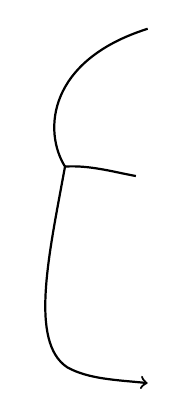
\begin{tikzpicture}[x=1cm,y=1cm]
\draw[thick,->] (1.45,4.5) .. controls (0.18,4.1) and (0.12,3.2) .. (0.40,2.75)
 .. controls (0.20,1.65) and (-0.06,0.52) .. (0.43,0.20)
 .. controls (0.70,0.05) and (1.06,0.04) .. (1.45,0);
\draw[thick] (0.40,2.75) .. controls (0.72,2.77) and (1.02,2.68) .. (1.30,2.63);
\end{tikzpicture}}

\scanpage{211}
\mspage{127}
% archive sheet number: 210
% element: text | top, introduction | Ces conditions sont satisfaites
Ces conditions sont satisfaites dans les \unsure{trois|deux} cas suivants :
% element: text | upper third, A | pi power equality
\begin{enumerate}[label={},leftmargin=2em]
\item[A)] $\pi^{\pi_0}=\pi$ (pour mémoire, c'est contenu dans 2\textsuperscript{o})
% element: text | upper third, B | Les familles épimorphiques
\item[B)] Les familles épimorphiques strictes dans $M$ sont épimorphiques strictes universelles.
% element: margin note | upper left, alongside B | Il suffit de supposer
\margin{Il suffit de supposer que les \unsure{épimorph.} stricts soient \unsure{stricts universels|universels} ; cf \unsure{compléments} 4.5.18.}
% element: text | upper middle, C | Les limites inductives
\item[C)] Les limites inductives filtrantes dans \deleted{$\unsure{C|E}$}$M$ commutent au chgt de base (ce qui est le cas notamment si les $\varinjlim$ filtrantes sont exactes \deleted{\unsure{finies}} à gauche).
\end{enumerate}
% element: margin note | middle left, diagonal | Je soupçonne que
% slanted
\margin{Je soupçonne que cette condition \unsure{revient|équivaut} à la \unsure{$=$|même|$\simeq$} condition sur $C$, pour les $\varinjlim$ filtrantes de cardinal $\leq\pi$.}
% element: text | middle, Remarque | La filtration de M
\uline{Remarque} La filtration de $M$ par les $\mathrm{Filt}'{}^\pi$ n'est autre que celle envisagée dans SGA 4 I 9.13, où on fait de plus l'hypothèse B) sur $M$, qui après-coup n'était plus tellement de mon goût. Toujours est-il que d'après (4.5.13.1), cette filtration se rapproche plus de la ``bonne'' filtration par les $M_\pi$, que celle que j'avais \unsure{cru|eu} \unsure{avoir raison de} lui préférer, celle par les $\mathrm{Filt}^\pi$. Elle a \inserted{d'ailleurs} sur cette dernière l'avantage, \inserted{dans le cas envisagé B)}, d'être une filtration cardinale \inserted{(ce qui n'est pas \unsure{même le cas|vrai} pour $\mathrm{Filt}^\pi$,} \deleted{Mais je} \deleted{\unsure{sauf erreur}} du moins s'il existe des cardinaux infinis $\pi>\pi_0$ avec $\pi^{\pi_0}\unsure{\neq|\not\geq|\not\leq}\pi$). Je soupçonne \deleted{\unsure{que}} maintenant qu'en général (et s'il existe des cardinaux infinis $\pi>\pi_0$ tels que $\pi^{\pi_0}\neq\pi$), en dehors des conditions A) B) C), la filtration par les $(\mathrm{Filt}'{}^\pi)$ n'est \uline{pas} une

\scanpage{212}
\mspage{128}
% archive sheet number: 211
% element: text | upper third, continuation | filtration cardinale
filtration cardinale. \deleted{\unsure{En}} En tous cas, 4.5.6 et la présente proposition, 3\textsuperscript{o}, montrent que si soit $(\mathrm{Filt}^\pi)_{\pi\unsure{\geq|>}\pi_2}$, soit $(\mathrm{Filt}'{}^\pi)_{\pi\geq\pi_2}$ est une filtration cardinale ($\pi_2$ étant un cardinal donné $\deleted{\unsure{\geq|\pi_2|\pi|\aleph}}\geq\unsure{\pi_0|\pi_1}$), alors elle coïncide avec la filtration par les $M_\pi$.

% element: text | middle, long parenthetical remark | Donc apparemment
Donc apparemment, dans tous les cas où je sais construire une filtration cardinale, sur un prototype du moins (i.e. sur une cat. $M$ stable par \inserted{petites} $\varinjlim$, \deleted{et} et dont les objets sont accessibles\unsure{\}|)}, \deleted{\unsure{et}} \deleted{\unsure{cela est|cela dit}} l'existence d'une filtration cardinale impliquant de plus celle d'une petite sous-cat. str. génératrice ...), celle-ci n'est autre que celle par les $M_\pi$ --- chose dont je ne m'étais pas aperçu en rédigeant SGA 4 I 9.

% element: text | lower third, proof heading | Dém de 4.5.13
\uline{Dém. de} 4.5.13.

% element: text | lower third, first assertion | Prouvons 1
Prouvons 1\textsuperscript{o}. On a les implications tautologiques
% element: diagram | lower third, six conditions | b double prime to b prime to b
\diagram{\begin{tikzcd}[ampersand replacement=\&]
b''\arrow[r,Rightarrow]\arrow[d,Rightarrow]\&b'\arrow[r,Rightarrow]\arrow[d,Rightarrow]\&b\arrow[d,Rightarrow]\\
a''\arrow[r,Rightarrow]\&a'\arrow[r,Rightarrow]\&a
\end{tikzcd}}
% element: margin note | lower right, beside diagram | compte tenu que C
\margin{compte tenu que $C$ est str. gén. dans $M$, donc $x\simeq\varinjlim_{i\in C/x}x_i$.}
% element: text | foot, concluding reduction | et pour prouver
et pour prouver l'équivalence de ces six conditions, il suffit de prouver
% element: diagram | bottom edge | a implies b double prime
\diagram{\begin{tikzcd}[ampersand replacement=\&]
a\arrow[r,Rightarrow]\&b''\unsure{\text{--}|.}
\end{tikzcd}}
